\documentclass[tikz]{standalone}
\usetikzlibrary{mindmap}
\begin{document}
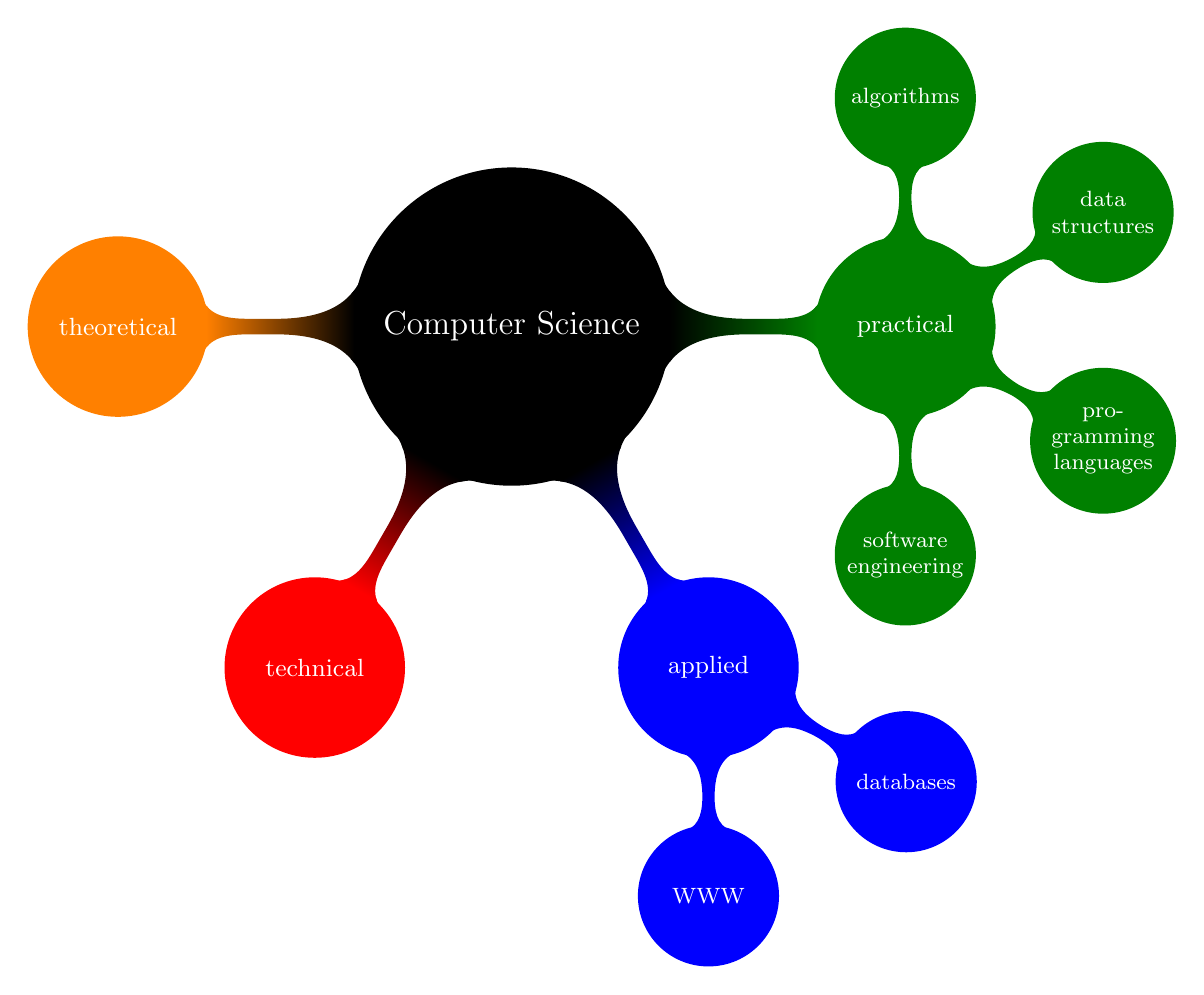
\begin{tikzpicture}
\path[mindmap,concept color=black, text=white]
	node[concept]	{Computer Science} [clockwise from=0]
		child[concept color=green!50!black]	{
			node[concept]	{practical}	[clockwise from=90]
			child	{	node[concept]	{algorithms}	}
			child	{	node[concept]	{data structures}	}
			child	{	node[concept]	{pro\-gramming languages}	}
			child	{	node[concept]	{software engineer\-ing}	}
		}
		child[concept color=blue]	{
			node[concept]	{applied}	[clockwise from=-30]
			child	{	node[concept]	{databases}	}
			child	{	node[concept]	{WWW}	}
		}
		child[concept color=red] {node[concept]	{technical}}
		child[concept color=orange]	{node[concept]	{
				theoretical}};
\end{tikzpicture}
\end{document}